%%%%%%%%%%%%%%%%%%%%%%%%%%%%%%%%%%%%%%%%%%%%%%%%%%%%%%%%
% This is just an example/guide for you to refer to when submitting manuscripts to Frontiers, it is not mandatory to use Frontiers .cls files nor frontiers.tex  %
% This will only generate the Manuscript, the final article will be typeset by Frontiers after acceptance.   
% When submitting your files, remember to upload this *tex file, the pdf generated with it, the *bib file (if bibliography is not within the *tex) and all the figures.
%%%%%%%%%%%%%%%%%%%%%%%%%%%%%%%%%%%%%%%%%%%%%%%%%%%%%%%%

%%% Version 3.4 Generated 2018/06/15 %%%
%%% You will need to have the following packages installed: datetime, fmtcount, etoolbox, fcprefix, which are normally inlcuded in WinEdt. %%%
%%% In http://www.ctan.org/ you can find the packages and how to install them, if necessary. %%%
%%%  NB logo1.jpg is required in the path in order to correctly compile front page header %%%

\documentclass[utf8]{frontiersSCNS} % for Science, Engineering and Humanities and Social Sciences articles
%\documentclass[utf8]{frontiersHLTH} % for Health articles
%\documentclass[utf8]{frontiersFPHY} % for Physics and Applied Mathematics and Statistics articles

%\setcitestyle{square} % for Physics and Applied Mathematics and Statistics articles
\usepackage{url,hyperref,lineno,microtype,subcaption}
\usepackage[onehalfspacing]{setspace}
\usepackage{multirow, graphicx} % added by authors for tables

\linenumbers % Leave a blank line between paragraphs instead of using \\

%%%%%%%%%%%%%%%%%%%%%%%%%%%%
%%% AUTHOR LIST
%%%%%%%%%%%%%%%%%%%%%%%%%%%%
\def\keyFont{\fontsize{8}{11}\helveticabold }
\def\firstAuthorLast{Rabonza {et~al.}} %use et al only if is more than 1 author
\def\Authors{Maricar L. Rabonza\,$^{1,2*}$, Yolanda C. Lin\,$^{3}$ and David Lallemant\,$^{1,2}$}

%%%%%%%%%%%%%%%%%%%%%%%%%%%%
%%% AFFILIATION
%%%%%%%%%%%%%%%%%%%%%%%%%%%%

\def\Address{
$^{1}$Asian School of the Environment, Nanyang Technological University, Singapore \\
$^{2}$Earth Observatory of Singapore, Nanyang Technological University, Singapore\\
$^{3}$Department of Geography and Environmental Studies, University of New Mexico, Albuquerque, NM, USA}
\def\corrAuthor{Maricar L. Rabonza}
\def\corrEmail{50 Nanyang Ave, Block N2-01c-63, 639798, Singapore
MARICARL001@e.ntu.edu.sg}

% Affiliations should be keyed to the author's name with superscript numbers and be listed as follows: Laboratory, Institute, Department, Organization, City, State abbreviation (USA, Canada, Australia), and Country (without detailed address information such as city zip codes or street names).
% If one of the authors has a change of address, list the new address below the correspondence details using a superscript symbol and use the same symbol to indicate the author in the author list.
% The Corresponding Author should be marked with an asterisk
% Provide the exact contact address (this time including street name and city zip code) and email of the corresponding author

%%%%%%%%%%%%%%%%%%%%%%%%%%%%%%%%%%%%%%%%%%%%%%%%%%%%%%%%|
%%% START OF DOCUMENT
%%%%%%%%%%%%%%%%%%%%%%%%%%%%
\begin{document}
\onecolumn
\firstpage{1}

\title[]{Learning from success, not catastrophe: using counterfactual analysis to highlight successful disaster risk reduction interventions} 

\author[\firstAuthorLast ]{\Authors} %This field will be automatically populated
\address{} %This field will be automatically populated
\correspondance{} %This field will be automatically populated
\extraAuth{}% If there are more than 1 corresponding author, comment this line and uncomment the next one.
%\extraAuth{corresponding Author2 \\ Laboratory X2, Institute X2, Department X2, Organization X2, Street X2, City X2 , State XX2 (only USA, Canada and Australia), Zip Code2, X2 Country X2, email2@uni2.edu}
\maketitle

%%%%%%%%%%%%%%%%%%%%%%%%%%%%|
%%% ABSTRACT
%%%%%%%%%%%%%%%%%%%%%%%%%%%%|
\begin{abstract}
%%% SUBMITTED ABSTRACT
In the aftermath of a disaster, news and research attention is focused almost entirely on catastrophic narratives and the various drivers that may have led to the disaster. Learning from failure is essential to preventing future disasters. However, hyperfixation on the catastrophe obscures potential successes at the local scale, which could serve as important examples and learning resource in effective risk mitigation. We propose the use of probabilistic downward counterfactual analysis to highlight effective risk mitigation actions that would otherwise remain unnoticed amidst a disaster. This approach uses counterfactual modelling of a past hazard event with consequences made worse (i.e. downward counterfactual) by the absence of the mitigation intervention. We further apply the probabilistic risk analysis framework to associate estimated probabilities to simulated counterfactual outcomes. We demonstrate the approach using a case study of the Nepal's School Earthquake Safety Program, implemented before the 2015 $M_{w}$ 7.8 Gorkha earthquake. We calculate the probabilistic number of lives saved during the earthquake as a result of the retrofitting of schools in Kathmandu Valley since 1999. The shift in focus from realised outcome to counterfactual alternative enables the quantification of the benefits of risk reduction activities amidst disaster. Such quantified counterfactual analysis can be used to celebrate successful risk reduction interventions, providing important positive reinforcement to decision-makers with political bravery to commit to the implementation of effective measures.

%%% KEYWORDS
\tiny \keyFont{ 
\section{Keywords:} counterfactual analysis, probabilistic risk, disaster risk reduction, risk framework, school earthquake safety} 
 % All article types: you may provide up to 8 keywords; at least 5 are mandatory.
\end{abstract}

%%%%%%%%%%%%%%%%%%%%%%%%%%%%|
%%% INTRODUCTION
%%%%%%%%%%%%%%%%%%%%%%%%%%%%|
\section{Introduction}
\label{section-intro}

Success in disaster risk management (DRM) means that natural hazard events do not become disasters, and communities continue to function and be resilient to shocks and stresses from hazards. Since the extent of a disaster can be characterised by loss of life, and disruptions to the physical, built and social environments, \citep{mileti1999disasters, smith2005through, moore1958tornadoes}, the extent of success of risk interventions manifest primarily as reduced impact. As such, success is measured as an \textit{absence} (e.g. no damage, fewer casualties, etc). This poses a challenge for recognising and incentivising important investments in DRM interventions since they are made invisible by their very nature.

In the aftermath of earthquakes, storms and floods, narratives of catastrophe dominate the interest of media, political and research communities. However, this hyper-fixation on the catastrophe can obscure important successes amid the broader disaster. Another challenge is to recognize successful interventions if the hazard they were designed for have not yet occurred. This happens when we rely on a disaster occurrence to make mitigation benefits visible. For extreme and rare hazard events for example, the benefits of risk reduction may be perceived far in the future only if the benefits manifest as reduced impact. Because of the significant time delay between the interventions and their benefits being manifested, the interventions could be seen as unsuccessful or squandered. 
These are two of the challenges described in \cite{lallemant_rabonza_gar_2022} where successful DRM interventions are made invisible: "invisible success in the midst of broader disaster", and "invisible success due to yet unrealised benefits." These 'invisible successes' of mitigation interventions are related to a cognitive tendency called 'outcome bias' - the tendency to judge the quality of a decision by the outcome alone \citep{robson_2019}. 

In this paper, we propose to address this bias through the use of probabilistic downward counterfactual analysis, and highlight effective risk reduction activities in terms of probabilistic lives saved. Two applications are presented to model how the consequences of a hazard event would be made worse by the absence of a risk reduction intervention (i.e. downward counterfactual). The first application estimates the benefits of an intervention in a past earthquake through comparison of fatalities modelled without the risk intervention and actual fatalities. The second application estimates the probabilistic benefits of a mitigation for a hazard that has not yet occurred. Instead of an actual past event, a hazard model is used to calculate the intervention's benefits.

The significance and novelty of this work is in shifting our perception of the benefits of risk reduction intervention, by using an appropriate counterfactual scenario as baseline against which to calculate and judge these benefits. Rather than focusing entirely on \textit{realised outcomes}, the analysis of \textit{counterfactual alternatives} shines light on the value of a mitigation intervention by demonstrating what would have been without such intervention. Downward counterfactual risk analysis has only so far been used to identify how much worse impacts could have been for the purpose of insurance, preparedness, or future mitigation \citep[e.g.][]{lin2020modeling, aspinall2019counterfactual, woo2019downward, woo2018counterfactual, shepherd2018storylines, woo2017reimagining, oughton2019stochastic, aspinall2019counterfactual}. This study pioneers a systematic approach to create incentives to good decision-making on the basis of probabilistic risk. The quantification of probabilistic lives saved by effective risk reduction programs in a major hazard event serves as a powerful indicator of the intervention's success that would otherwise remain unnoticed amidst a disaster. In addition, the calculated probabilistic benefits over the lifetime of an intervention provides important incentive and encouragement to decision-makers committed to implement effective measures even if the benefits are not materialized yet by the occurrence of a hazard event. Altogether, this work is a new domain of application of counterfactual analysis with much potential across the broad spectrum of hazards. 

The proposed framework has significant implications to multiple potential stakeholders. For policymakers, there is currently little political capital gained from investing in resilience if the benefits of such investments are invisible. By having the benefits of their risk reduction investments visible to their constituents, policymakers will be incentivised for risk-informed decision-making. For donors and funders, this framework would enable them to monitor progress in terms of probabilistic impacts reduced, even if such benefits remain unrealized until a disaster strikes. For disaster risk management practitioners, while it is important to learn from failures, it is equally important to learn from successes, and share them broadly so they can be emulated, scaled, and adapted in other contexts where they are needed. Importantly, it also provides a mechanism to recognise and elevate the important, humble, long-term and dedicated work conducted by many to keep our communities safe, even when their work is unseen.

The paper is organized as follows. Section \ref{section-counter} introduces the proposed framework in the context of risk analysis and probabilistic modelling. In Section \ref{section-retrofit-program}, we describe the earthquake risk intervention that will be the focus of our two applications: the school earthquake retrofitting program in Nepal, implemented before the 2015 $M_{w}$ 7.8 Gorkha earthquake, herein called Gorkha earthquake. In the subsequent sections, we present the data (Section \ref{section-data}), methods (Section \ref{section-methods}) and results (Section \ref{section-results}) for two applications that shed light on the benefits of the retrofitting program. The first application calculates the probabilistic number of lives saved during the Gorkha earthquake as a result of the retrofitting of schools in Kathmandu valley since 1997. The second application calculates future probabilistic lives saved by the retrofitting program based on a probabilistic seismic hazard model for Kathmandu Valley. This is followed by discussion (Section \ref{section-discuss}) and conclusion (Section \ref{section-conclusion}).

%%%%%%%%%%%%%%%%%%%%%%%%%%%%|%%%%%%%%%%%%%%%%%%%%%%%%%%%%|
%%% COUNTERFACTUAL ANALYSIS
%%%%%%%%%%%%%%%%%%%%%%%%%%%%|%%%%%%%%%%%%%%%%%%%%%%%%%%%%|
\section{Counterfactual risk analysis framework}
\label{section-counter}

Counterfactual analysis allows the exploration of alternative branches of history by creating what-if scenarios \citep{Todorova_2015, lewis2005tbe}. To apply counterfactual analysis in disaster risk analysis, the realised event and the counterfactual are characterised in terms of their risk parameters \citep[e.g.][]{lin2020modeling, lallemant_rabonza_gar_2022}.  Disaster risk is typically characterised as a function of: (a) Hazard, the likelihood of potential damaging events, (b) Exposure, the characteristics of assets such as people, buildings and infrastructure and (c) Vulnerability, the susceptibility of the exposed assets to sustain impact for a given hazard intensity \citep{UNISDRterms2009}. Therefore, the realised event's impact is expressed as:
    \begin{equation}\label{eq:realised}
        I_{realised} = f \left( \theta_H, \theta_E, \theta_V \right),
    \end{equation}
where $\theta_H$, $\theta_E$, and $\theta_V$ are the hazard, exposure and vulnerability parameters consecutively. Modifications ($\delta_{.}$) of one or multiple parameters that define the realised event allows one to define the impact of a counterfactual event:
    \begin{equation}\label{eq:counterfactual_risk}
        I_{counterfactual} = f \left( \theta_H + \delta_H, \theta_E + \delta_E, \theta_V + \delta_V \right),
    \end{equation}
To study a range of counterfactual events, the parameters in Equation \ref{eq:counterfactual_risk} are treated as random variables with known probability distributions. The joint-probability of the parameters then defines the probability of the counterfactual. In practice, this is calculated using a simulation (e.g. Monte-Carlo simulation) since there is rarely an analytical solution. The benefits ($B$) of effective risk mitigation is obtained by comparing the distribution of counterfactual impacts to the realised impacts (Equation \ref{eq:benefits} and Figure \ref{fig:conceptual_diagram}). 
    \begin{equation} \label{eq:benefits}
        B = I_{realised} - I_{counterfactual}
    \end{equation}


%%%%%%%%%%%%%%%%%%%%%%%%%%%%|%%%%%%%%%%%%%%%%%%%%%%%%%%%%|
%%% SCHOOLS RETROFIT
%%%%%%%%%%%%%%%%%%%%%%%%%%%%|%%%%%%%%%%%%%%%%%%%%%%%%%%%%|
\section{Invisible success of seismically retrofitting school in Nepal}
\label{section-retrofit-program}

In this paper, we implement the proposed framework to highlight invisible benefits of effective earthquake risk mitigation. Specifically, we focus on one of the most significant risk interventions in the recent years that conducted improved construction practices - the seismic retrofitting of school buildings in Nepal. The program's success in the midst of the 2015 Gorkha earthquake, and its benefits due to yet unrealised benefits until the occurrence of a future large earthquake are both made invisible. 

The safety of school buildings has always been of specific concern, reflecting a particular societal care for the lives of young people. School buildings also serve important recovery functions following disaster such as congregation points for the community, and sites for emergency shelters and health services \citep{dixit2014public}. 

School buildings in Nepal are recognized to be at high risk amidst the region's high seismicity from the convergence of the Indian tectonic plate with the Eurasian plate, and due to informal construction practices done without engineering guidance \citep{marasini2020}. Damage to school buildings was extensive from large earthquakes in recent history - the 1988 $M_{w}$ 6.6 Udayapur earthquake \citep{gupta1988report}, and the 2011 $M_{w}$ 6.9 Sikkim/Nepal border earthquake \citep{rai2012reconnaissance}. The 2015 Gorkha earthquake is a unique example in terms of damage to schools because the earthquake happened on a Saturday, whilst the school was not in session. Had the earthquake hit on a school day, over one million students would have been affected \citep{dixit2014public}.

Seismic retrofitting of school buildings started in 1997 through the leadership of the National Society for Earthquake Technology (NSET) as part of the Nepal's School Earthquake Safety Program (SESP)  \citep{marasini_2019}. By the time of the Gorkha earthquake in 2015, 300 schools had been retrofitted, 160 of which were in the most affected districts (78 in Kathmandu). It was a big achievement that none of the schools retrofitted under SESP collapsed or needed major repairs after the earthquake. Because the buildings were found to be structurally sound, all the retrofitted buildings served as safe shelters and required fewer temporary classrooms \citep{marasini_2019}. 

Following the direction of SESP towards safe learning facilities, the Government of Nepal aims to achieve minimum school safety criteria nationwide by 2030 through the Comprehensive School Safety Master Plan developed by Nepal's Ministry of Education, Science and Technology \citep{cehrdc2018} based on the global Comprehensive School Safety Framework \citep{unisdr2017}. Recognizing the need to strengthen more than 60,000 school buildings all over Nepal \citep{marasini2020}, one of the activities in the Master Plan is to retrofit school buildings in earthquake-affected areas.

%%%%%%%%%%%%%%%%%%%%%%%%%%%%|%%%%%%%%%%%%%%%%%%%%%%%%%%%%|
%%% DATA
%%%%%%%%%%%%%%%%%%%%%%%%%%%%|%%%%%%%%%%%%%%%%%%%%%%%%%%%%|
\section{Data}
\label{section-data}

\subsection{Exposure: Building portfolio characteristics}

    We use data of 5,011 school buildings in Kathmandu Valley that consist of 4,941 non-retrofitted buildings and 70 buildings retrofitted for earthquake resilience under SESP. Shown in Figure \ref{fig:datacase1} is a map of the 70 retrofitted schools, and in Figure \ref{fig:datacase2} is a map of all 5011 school buildings in the database. The dataset was produced through partnership of the Open Data for Resilience Initiative and the Government of Nepal with support from Kathmandu Living Lab \citep{opendri_2012}. The 70 retrofitted schools in the dataset is part of the 78 retrofitted schools surveyed by NSET in Kathmandu Valley's affected areas \citep{marasini_2019}. Key attributes of each school building are extracted such as the coordinates, number of daytime occupants (i.e. occupants in a school day), number of floors and the material used for construction. The daytime occupants for the 70 retrofitted schools range from 1 to 800 with a mean of 134, whereas the daytime occupants for the 5011 school buildings range from 1 to 2000 with a mean of 120.
    
\subsection{Vulnerability: Building fragility}

    Fragility curves represent the probability of a certain level of damage to buildings for a given earthquake intensity ($IM$) and building class. A fragility function for building collapse ($P(Collapse|IM)$), obtained through a generalized linear model based regression, reduces to Equation \ref{eq:fragility} where $\Phi$ is the cumulative distribution function of the standard normal distribution, and $\alpha$ and $\beta$ are the maximum likelihood parameter estimates for the regression model \citep{Lallemant2015}.

        \begin{equation}\label{eq:fragility}
            P(Collapse|IM) = \Phi(\alpha + \beta log(IM))
        \end{equation}

     Non-retrofitted school buildings are assigned to building classes B-, B, K5, or C2 as defined by \cite{jica2002study}'s survey of buildings in Kathmandu Valley before the Gorkha Earthquake (see fragility curves in Figure \ref{fig:frag_curves} and parameters in Table \ref{tab:frag_params}). Fragility curves for the retrofitted buildings are not available, so we instead adopt the fragility curve for a specially designed reinforced concrete (RC) building (Building class C3).
    
     Had the 70 school buildings not been retrofitted, majority of them consist of Type B buildings, which are 1-3 storey buildings made of mud mortar or cement mortar (see distribution of non-retrofitted building classes in Figure \ref{fig:datacase1}). Similarly, majority of the 5,011 buildings in the dataset are Type B buildings (see Figure \ref{fig:datacase2}).

\subsection{Hazard models}

To best represent the shaking at the school buildings' sites at the time of the 2015 Gorkha earthquake, we use peak ground acceleration (PGA) values produced with stochastic simulations (high frequency) for Kathmandu (Figure \ref{fig:datacase1}). This simulation method is well-accepted by the strong-motion community because wave propagation and source radiation tend to become more stochastic at high frequencies. This hazard model for the 2015 Gorkha earthquake was selected for this study because the location of sources of the high-frequency energy (strong-motion generation areas) is a critical factor in the relatively low damage phenomenon observed in Kathmandu Valley during the 2015 Gorkha earthquake \citep{gallovivc2016modeling, koketsu2016widespread}, aside from effects of site conditions and rupture directivity \citep{dixit2015strong, rajaure2017characterizing, gallovivc2016modeling, koketsu2016widespread}. In addition, most ground-motion prediction equations (GMPEs) do not account for Kathmandu Valley's low damage phenomenon \citep{dixit2015strong, martin2015ground, hough2016comparison, takai2016strong}. With this hazard model, PGA values at the location of the retrofitted buildings range from 0.065 to 0.149 g, and comes in a resolution of 0.0167 degrees, or around 1.85km.  More details about the PGA data are summarized in \cite{chen20192015} and its companion paper, \cite{wei20182015}.

Another hazard model we use for this paper is the probabilistic seismic hazard analysis (PSHA) for the region where the school building dataset is located (Figure \ref{fig:datacase2}). We adopt \cite{stevens2018probabilistic}'s PSHA model for Kathmandu that incorporates detailed geometry of the Main Himalayan thrust, site effects, and most appropriate GMPEs informed by observed PGA and damaged patterns. The probabilistic hazard model was generated using the OpenQuake engine \citep{pagani2014openquake, silva2014development}. We use PGA values corresponding to a 10\% probability of exceedance in 50 years from \cite{stevens2018probabilistic}'s PSHA with a resolution of 0.0083 degrees (around 0.9 km). Including site effects, the school buildings are expected to have a 10\% probability of exceeding shaking of 0.506 to 0.649g in any 50 year period. 

%%%%%%%%%%%%%%%%%%%%%%%%%%%%|%%%%%%%%%%%%%%%%%%%%%%%%%%%%|
%%% METHODS
%%%%%%%%%%%%%%%%%%%%%%%%%%%%|%%%%%%%%%%%%%%%%%%%%%%%%%%%%|
\section{Methods}
\label{section-methods}

%%%%%%%%%%%%%%%%%%%%%%%%%%%%|
\subsection{Estimating lives saved amidst 2015 Gorkha earthquake}
\label{section-case1}

This case study imagines the scenario: What if the 2015 Gorkha earthquake happened on a school day, and the seismic retrofitting program had not been implemented? With the counterfactual risk framework, we estimate the building collapse for a realised case where the 70 school buildings were retrofitted, and a counterfactual case where these buildings are not retrofitted using the data shown in Figure \ref{fig:datacase1}. To explore the impact of reduced fragility from the program to the final risk results, the hazard and exposure footprint remain static, i.e. we use the same hazard data and building portfolio characteristics (number of schools, location, daytime occupancy) for the two scenarios.

The probability of exceeding a school building's collapse damage state is estimated based on the peak ground acceleration (PGA) at the site, daytime occupancy, building class based on construction typology, and collapse fragility curves. The realised scenario uses fragility data for retrofitted buildings, whereas the counterfactual scenario uses fragility curves for non-retrofitted building classes. A Monte Carlo simulation of Bernoulli trials then generates a distribution of number of collapsed buildings in the realised case and counterfactual case. We can estimate the number of avoided building collapse by comparing the building collapse between the realised and counterfactual scenario. 

We further extend the benefit calculation beyond avoided building collapse, and quantify probabilistic lives saved, using the buildings' occupancy data and a 20\% fatality rate from NSET's recommendation for RC and masonry building class \citep{nset2000}. Estimated fatalities for the counterfactual scenario represent the distribution of probabilistic lives lost had the school buildings not been retrofitted. The estimated fatalities for the realised scenario is a model of probabilistic lives lost as it happened in reality. Finally, we interpret the probabilistic lives saved by the intervention as the difference between the means of the distributions of the simulated fatalities in the counterfactual and realised scenario. The estimated fatality from the simulation of the realised event can be compared to reported post-event casualty records to validate the modelled casualties. All model runs are performed using R environment and programming language \citep{team2013r} and resulting figures are produced using the packages ggplot2 \citep{ggplot22016} and ggridges \citep{ggridges2021} (source code available at https://github.com/ntu-dasl-sg/frontiers2021-PLS).

%%%%%%%%%%%%%%%%%%%%%%%%%%%%|
\subsection{Estimating lives saved throughout the program's lifetime}
\label{section-case2}

Scaling up the retrofitting program to more than 60,000 school buildings in Nepal under the Comprehensive School Safety Master Plan will significantly enhance the schools' resilience to earthquakes \citep{cehrdc2018}. In this analysis, we imagine the downward counterfactual: 'What if the school seismic retrofitting program was never and will never be implemented to thousands of school buildings in Kathmandu Valley?' Given the seismic hazard of Nepal, what are the estimated school-building collapse rates and fatalities expected in the next decades? The aim of this analysis is to demonstrate how to use counterfactual analysis to highlight the probabilistic benefits of the school retrofit program.

For this case study, we make use of a building portfolio data that consists of 5011 school buildings in Kathmandu Valley - a subset of the 60,000 school buildings that is aimed to be strengthened for earthquake resilience (see Figure \ref{fig:datacase2}). In this approach, we imagine a certain point in time in the future where the Government of Nepal will finish retrofitting the 5011 school buildings in our study area. With this assumption, the actual scenario for our analysis means that all school buildings in our dataset will be fully retrofitted. Our counterfactual scenario represents, that at this point in time in the future, all the school buildings were never retrofitted because SESP and the Comprehensive School Safety Master Plan is non-existent.

The analysis is first-order and comes with simplifications. For the two scenarios, we make use of the same exposure data and hazard model (10\% probability of exceedance in 50 years). For simplicity of analysis, we assume that exposure remains constant over time, meaning the number of schools and its occupants do not change. The only difference between the two scenarios is the forecasted building stock vulnerability at the end of the program's lifetime. For the actual scenario, all 5,011 buildings are retrofitted with a C3 building class' fragility. Whereas for the counterfactual scenario, all buildings will be assigned non-retrofitted building classes, namely, B-, B, K5 and C2. To clarify, the counterfactual assumes that the 70 buildings already retrofitted at the time of the building survey are non-retrofitted, as if the retrofit program didn't exist. Using the proposed counterfactual risk framework, we estimate the probabilistic building collapse for the two scenarios mentioned. We implement the fatality calculation approach used in the first case study to obtain a distribution of probabilistic fatalities.

The simplifications are sufficient to demonstrate how the framework can highlight the benefits of the school retrofit program even if an earthquake event hasn't happened yet. A modeller with more information about time-dependent exposure (e.g. growing building portfolio) and vulnerability (e.g. sequential retrofitting) can opt to implement this methodology at multiple points in time to get time-dependent building collapse and study long term risk \citep{rabonza2019accounting}. 

%%%%%%%%%%%%%%%%%%%%%%%%%%%%|%%%%%%%%%%%%%%%%%%%%%%%%%%%%|
%%% RESULTS
%%%%%%%%%%%%%%%%%%%%%%%%%%%%|%%%%%%%%%%%%%%%%%%%%%%%%%%%%|
\section{Results}
\label{section-results}

\subsection{Lives saved amidst 2015 Gorkha earthquake}

Our probabilistic analysis show that in the realised scenario (all buildings retrofitted), an average of 3 out of the 70 school buildings collapsed, whereas for the counterfactual case (all buildings non-retrofitted), an average of 12 out of the 70 school buildings collapsed. Based on these results, 9 school buildings likely avoided collapse thanks to the retrofitting intervention (Figure S1). The simulation of the realised fatalities during the Gorkha earthquake shows a mean of 74 fatalities, whereas counterfactual fatalities have an average of 300 (Figure \ref{fig:results_case1}). By comparing the fatalities from the two scenarios, we estimate that the lives of approximately 226 school occupants were saved in Kathmandu by the retrofit of the 70 schools.

\subsection{Lives saved throughout the program's lifetime}

Our model forecasts that the collapse of 2,490 buildings are likely to be avoided if all the 5,011 buildings will be retrofitted based n PGA values for 10\% probability of exceedance in 50 years (Figure S2). Our simulation for the 'actual' scenario where all buildings are retrofitted shows a mean of 20,207 fatalities whereas the fatalities from the counterfactual simulation has a mean of 79,529. Based on the counterfactual analysis, 59,322 lives will be saved by the retrofitting of the 5,011 buildings (Figure \ref{fig:results_case2}).


%%%%%%%%%%%%%%%%%%%%%%%%%%%%|%%%%%%%%%%%%%%%%%%%%%%%%%%%%|
%%% DISCUSSION
%%%%%%%%%%%%%%%%%%%%%%%%%%%%|%%%%%%%%%%%%%%%%%%%%
\section{Discussion}
\label{section-discuss}
%%%%%%%%%%%%%%%%%%%%%%%%%%%%|
\subsection{Counterfactual analysis to celebrate probabilistic lives saved}

We demonstrated two applications of the probabilistic downward counterfactual risk analysis to (1) celebrate lives saved by an intervention amidst a past event, and (2) forecast lives saved throughout the intervention's lifetime with the use of a probabilistic hazard model. The two applications show that even in the midst of a tragic disaster, or even if a hazard event hasn't happened yet, there are often successes in risk reduction intervention to celebrate. The counterfactual analysis showed that hundreds of lives are estimated to be saved because of the government-led retrofitting of 70 school buildings in the dataset. The program's benefit is obscured further because the Gorkha earthquake happened on a day without school sessions. Our second application also estimated that tens of thousand of fatalities are likely to be avoided once the 5,011 school buildings in our dataset are retrofitted. 

Although it is known that none of the retrofitted schools collapsed based on damage assessments after the Gorkha earthquake, the number of fatalities in the 70 school buildings is unknown \citep{marasini_2019}. Assuming that the actual casualties in these buildings are lower than the mean of our fatality estimates (74), it would likely be due to the fragility data underestimating the structural performance of the buildings.

%%%%%%%%%%%%%%%%%%%%%%%%%%%%|
\subsection{Risk benefit metric}
In our demonstrations, the risk benefit of DRM intervention is measured in terms of a reduction in loss of life - the first target metric within the Sendai Framework For Disaster Risk Reduction \citep{united2015sendai}. A risk benefit metric in financial units can also be used, as with typical cost-benefit analysis. However such analysis tend to highlight interventions that effectively protect high-value areas instead of high-vulnerability areas, which exacerbates inequities \citep{markhvida_quantification_2020, lallemant2020informatics}. 

More alternative risk benefit metrics for this analysis include the number of displaced people, business downtime, damage to buildings and cultural heritage, psychological distress and more. For the Nepal case study for example, the benefits of the retrofitting go well beyond the reduced physical vulnerability of the buildings. Retrofitted schools served as immediate community shelter, field hospitals and relief centers. Classes in the retrofitted buildings were operated without fear, resulting to less demand for temporary classrooms \citep{marasini2020}. Loss-avoidance is not the only invisible benefit of disaster mitigation, and benefits of DRM interventions go beyond reduction of impact. Certain intervention designs can have co-benefits that are social (e.g. more leisure parks), environmental (e.g. wetland afforestation), political (e.g. better governance), or economic (e.g. better agriculture production) \citep{Tanner2015}.

%%%%%%%%%%%%%%%%%%%%%%%%%%%%|
\subsection{First order approach}

The analyses and estimates of lives saved presented are first order and serve as proof of concept of the counterfactual framework to highlight successes in DRM. Following are limitations that need to be noted for future work:

\begin{itemize}
    \item 
    The analysis did not account for fatalities from partially collapsed buildings. To account for this, one may use NSET's recommendation to use a 10\% fatality rate for heavily damaged buildings \citep{nset2000}
    \item
    The building portfolio dataset we use in the two case studies is only a subset of all the schools within the study area. The dataset used for the first case study (Section \ref{section-case1}) contains only 70 out of the 78 retrofitted schools in Kathmandu. For the second case study (Section \ref{section-case2}), we also did not include school building data that has no information on the occupancy and construction material.
    \item
    For the second case study, the assumption that the goal of the Government of Nepal is to finish retrofitting the 5,011 buildings in our dataset is not necessarily reflective of their exact plan of action. Rather, the assumption is a choice of the authors to demonstrate the framework in a simple and straightforward manner.
\end{itemize}

In an attempt to explore how different the casualty estimates would be for different hazard models for the 2015 Gorkha earthquake, we repeated the analysis in Section \ref{section-case1} using a PGA map from the USGS ShakeMap \citep{wald2007topographic}. Looking at the results in Figure S3, using ShakeMap results to 355 lives saved. This is only a simple exploration using a different hazard model, and not a full sensitivity analysis.

%%%%%%%%%%%%%%%%%%%%%%%%%%%%|
\subsection{Extending to other domains of hazard and interventions}

Probabilistic downward counterfactual risk analysis has potential for application to other hazards. A key step of the framework is to identify which risk component the intervention influences. Earthquake risk reduction, for example, influences either the reduction of exposure or vulnerability. Measures such as restricting development in high-hazard zones decrease exposure, whereas better construction standards decrease the structural vulnerability of buildings and infrastructure.

Beyond earthquake risk reduction, the proposed framework can also be used in other domains of hazard. Following are few selected examples of natural hazards and corresponding interventions that could be celebrated using counterfactual analysis. Enclosed in parenthesis are the risk component/s that the intervention influences.

\begin{enumerate}

    \item \textbf{Earthquake}
    \begin{itemize}
            \item Reconstruction and seismic retrofit (Vulnerability)
            \item Construction inspection (Vulnerability)
            \item Preparedness exercises (Exposure, Vulnerability)
    \end{itemize}
    
    \item \textbf{Tropical cyclone and Tsunami}
    \begin{itemize}
            \item Early warning system and timely announcements (Exposure)
            \item Evacuation and provision of temporary shelters (Exposure and Vulnerability)
            \item Public awareness about the hazard (Exposure and Vulnerability)
    \end{itemize}
    
    \item \textbf{Flood}
    \begin{itemize}
            \item Limiting urban development in flood-prone zones (Exposure, Vulnerability)
            \item Enhanced flood management infrastructure (Exposure, Hazard)
            \item Timely emergency response (Vulnerability, Exposure)
    \end{itemize}

    \item \textbf{Landslides}
    \begin{itemize}
            \item Early warning system via geodynamic monitoring (Exposure)
            \item Mitigation infrastructure, e.g. drainage systems (Exposure, Hazard)
    \end{itemize}

    \item \textbf{Wildfires}
    \begin{itemize}
            \item Early warning system via dynamic weather forecasts (Exposure)
    \end{itemize}

\end{enumerate}

%%%%%%%%%%%%%%%%%%%%%%%%%%%%|%%%%%%%%%%%%%%%%%%%%%%%%%%%%|
%%% CONCLUSION
%%%%%%%%%%%%%%%%%%%%%%%%%%%%|%%%%%%%%%%%%%%%%%%%%%%%%%%%%|
\section{Conclusion}
\label{section-conclusion}

In a field focused on long-term resilience to rare (i.e. volatile) hazard events, perceptions are biased by realised outcomes. Perceiving no impacts when DRM work is so successful can result to policy makers and society at large to undervalue the importance of proactive intervention. Shedding light on successes and ‘what might have been’ not only recognizes the outstanding work of those in the industry but is also a crucial component of encouraging decision-makers to continue investment in measures that keep our communities and world safe. 

We highlight the need to celebrate the often invisible successes of disaster risk reduction interventions, in order to incentivise, better learn and replicate investments in such interventions. We further propose and demonstrate the use of counterfactual analysis risk framework to identify, quantify and highlight these invisible successes. The framework demonstrates that judgement of a risk reduction intervention should be based on a broad exploration of possible outcomes, not only on specific outcomes.

% All data and code in Github
% https://github.com/maricarl001/prob-lives-saved

%%%%%%%%%%%%%%%%%%%%%%%%%%%%%%%%%%%%%%%%%%%%%%%%%%%%%%%%|
%%% ADDITIONAL REQUIREMENTS
%%%%%%%%%%%%%%%%%%%%%%%%%%%%%%%%%%%%%%%%%%%%%%%%%%%%%%%%|

%%%%%%%%%%%%%%%%%%%%%%%%%%%%
\section*{Conflict of Interest Statement}

The authors declare that the research was conducted in the absence of any commercial or financial relationships that could be construed as a potential conflict of interest.

% All financial, commercial or other relationships that might be perceived by the academic community as representing a potential conflict of interest must be disclosed. If no such relationship exists, authors will be asked to confirm the following statement: 

%%%%%%%%%%%%%%%%%%%%%%%%%%%%
\section*{Author Contributions}

All authors contributed to the conceptualisation and design of the study. DL conceived of the idea of celebrating successes in disaster risk reduction using counterfactual analysis. MR and YL designed the analysis of the first case study. MR designed the analysis of the second case study. MR took the lead in writing the manuscript and performed analyses for the case studies. YL and DL provided critical feedback that shaped the research, analysis and manuscript.

% The Author Contributions section is mandatory for all articles, including articles by sole authors. If an appropriate statement is not provided on submission, a standard one will be inserted during the production process. The Author Contributions statement must describe the contributions of individual authors referred to by their initials and, in doing so, all authors agree to be accountable for the content of the work. Please see  \href{http://home.frontiersin.org/about/author-guidelines#AuthorandContributors}{here} for full authorship criteria.

%%%%%%%%%%%%%%%%%%%%%%%%%%%%
\section*{Funding}
This project is supported by the National Research Foundation, Prime Minister’s Office, Singapore under the NRF-NRFF2018-06 award, the Earth Observatory of Singapore, the National Research Foundation of Singapore, and the Singapore Ministry of Education under the Research Centers of Excellence initiative. MR is supported by a PhD scholarship from the Earth Observatory of Singapore.

%%%%%%%%%%%%%%%%%%%%%%%%%%%%
\section*{Acknowledgments}
We thank Dr. Nama Budhathoki, Kathmandu Living Labs and the GFDRR Open Data for Resilience Initiative for data on school buildings in Nepal. We also thank Dr. Shengji Wei and Dr. Meng Chen for data and information on the stochastic ground simulations in Kathmandu for the 2015 Gorkha earthquake.

%%%%%%%%%%%%%%%%%%%%%%%%%%%%
\section*{Supplemental Data}

% See Overleaf for Supplementary Figures: http://home.frontiersin.org/about/author-guidelines#SupplementaryMaterial

%  \href{http://home.frontiersin.org/about/author-guidelines#SupplementaryMaterial}{Supplementary Material} should be uploaded separately on submission, if there are Supplementary Figures, please include the caption in the same file as the figure. LaTeX Supplementary Material templates can be found in the Frontiers LaTeX folder.


% %%%%%%%%%%%%%%%%%%%%%%%%%%%%
\section*{Data Availability Statement}
The original contributions presented in the study are included in the article. Further inquiries can be directed to the corresponding author/s.
% The datasets [GENERATED/ANALYZED] for this study can be found in the [NAME OF REPOSITORY] [LINK].
% Please see the availability of data guidelines for more information, at https://www.frontiersin.org/about/author-guidelines#AvailabilityofData

%%%%%%%%%%%%%%%%%%%%%%%%%%%%
%%% BIBLIOGRAPHY
%%%%%%%%%%%%%%%%%%%%%%%%%%%%
\bibliographystyle{frontiersinSCNS_ENG_HUMS} % for Science, Engineering and Humanities and Social Sciences articles, for Humanities and Social Sciences articles please include page numbers in the in-text citations
%\bibliographystyle{frontiersinHLTH&FPHY} % for Health, Physics and Mathematics articles
\bibliography{test}
%%% Make sure to upload the bib file along with the tex file and PDF
%%% Please see the test.bib file for some examples of references

%%%%%%%%%%%%%%%%%%%%%%%%%%%%
%%% FIGURES
%%%%%%%%%%%%%%%%%%%%%%%%%%%%

\section*{Figure captions}

\begin{figure}[h!] 
\begin{center}
    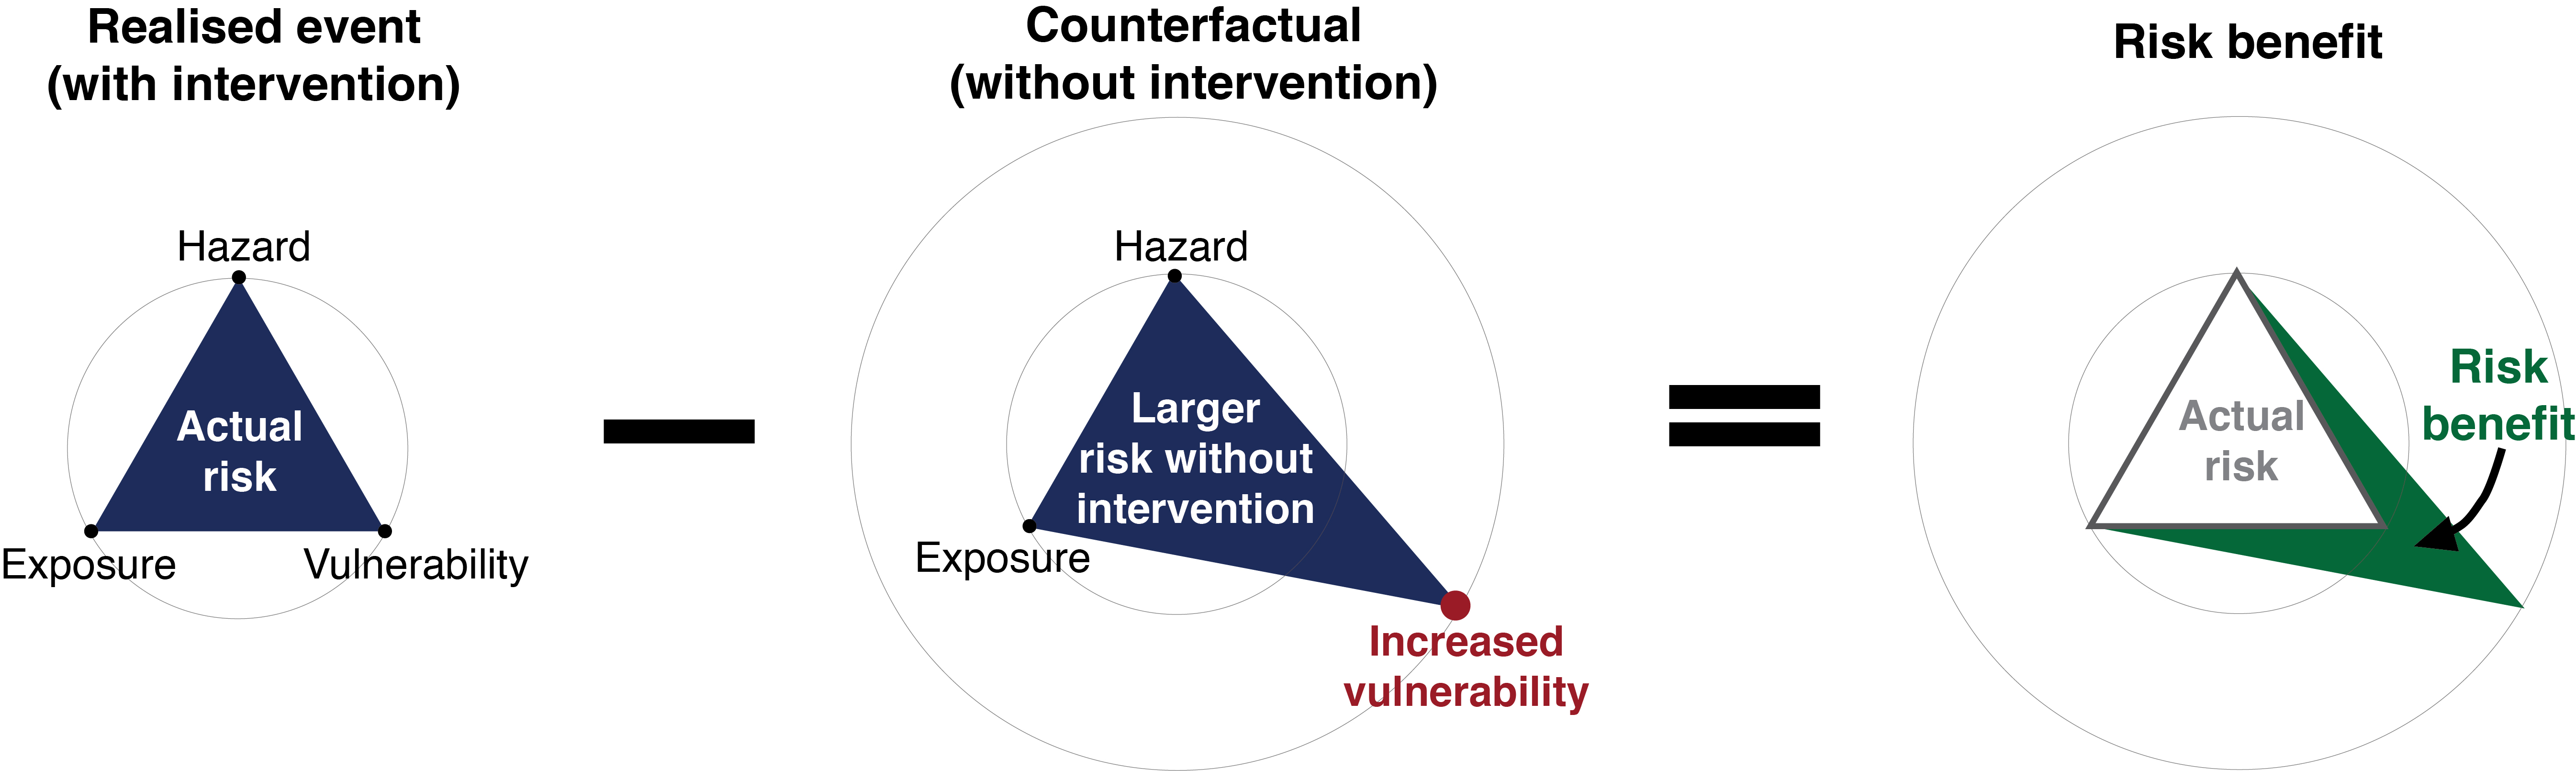
\includegraphics[width=\textwidth]{Figures/concept-diagram.jpg}
    \caption{The concept of the counterfactual risk analysis framework for quantifying the probabilistic benefits of effective risk reduction}
    \label{fig:conceptual_diagram}
\end{center}
\end{figure}

\begin{figure}[h!] 
\begin{center}
    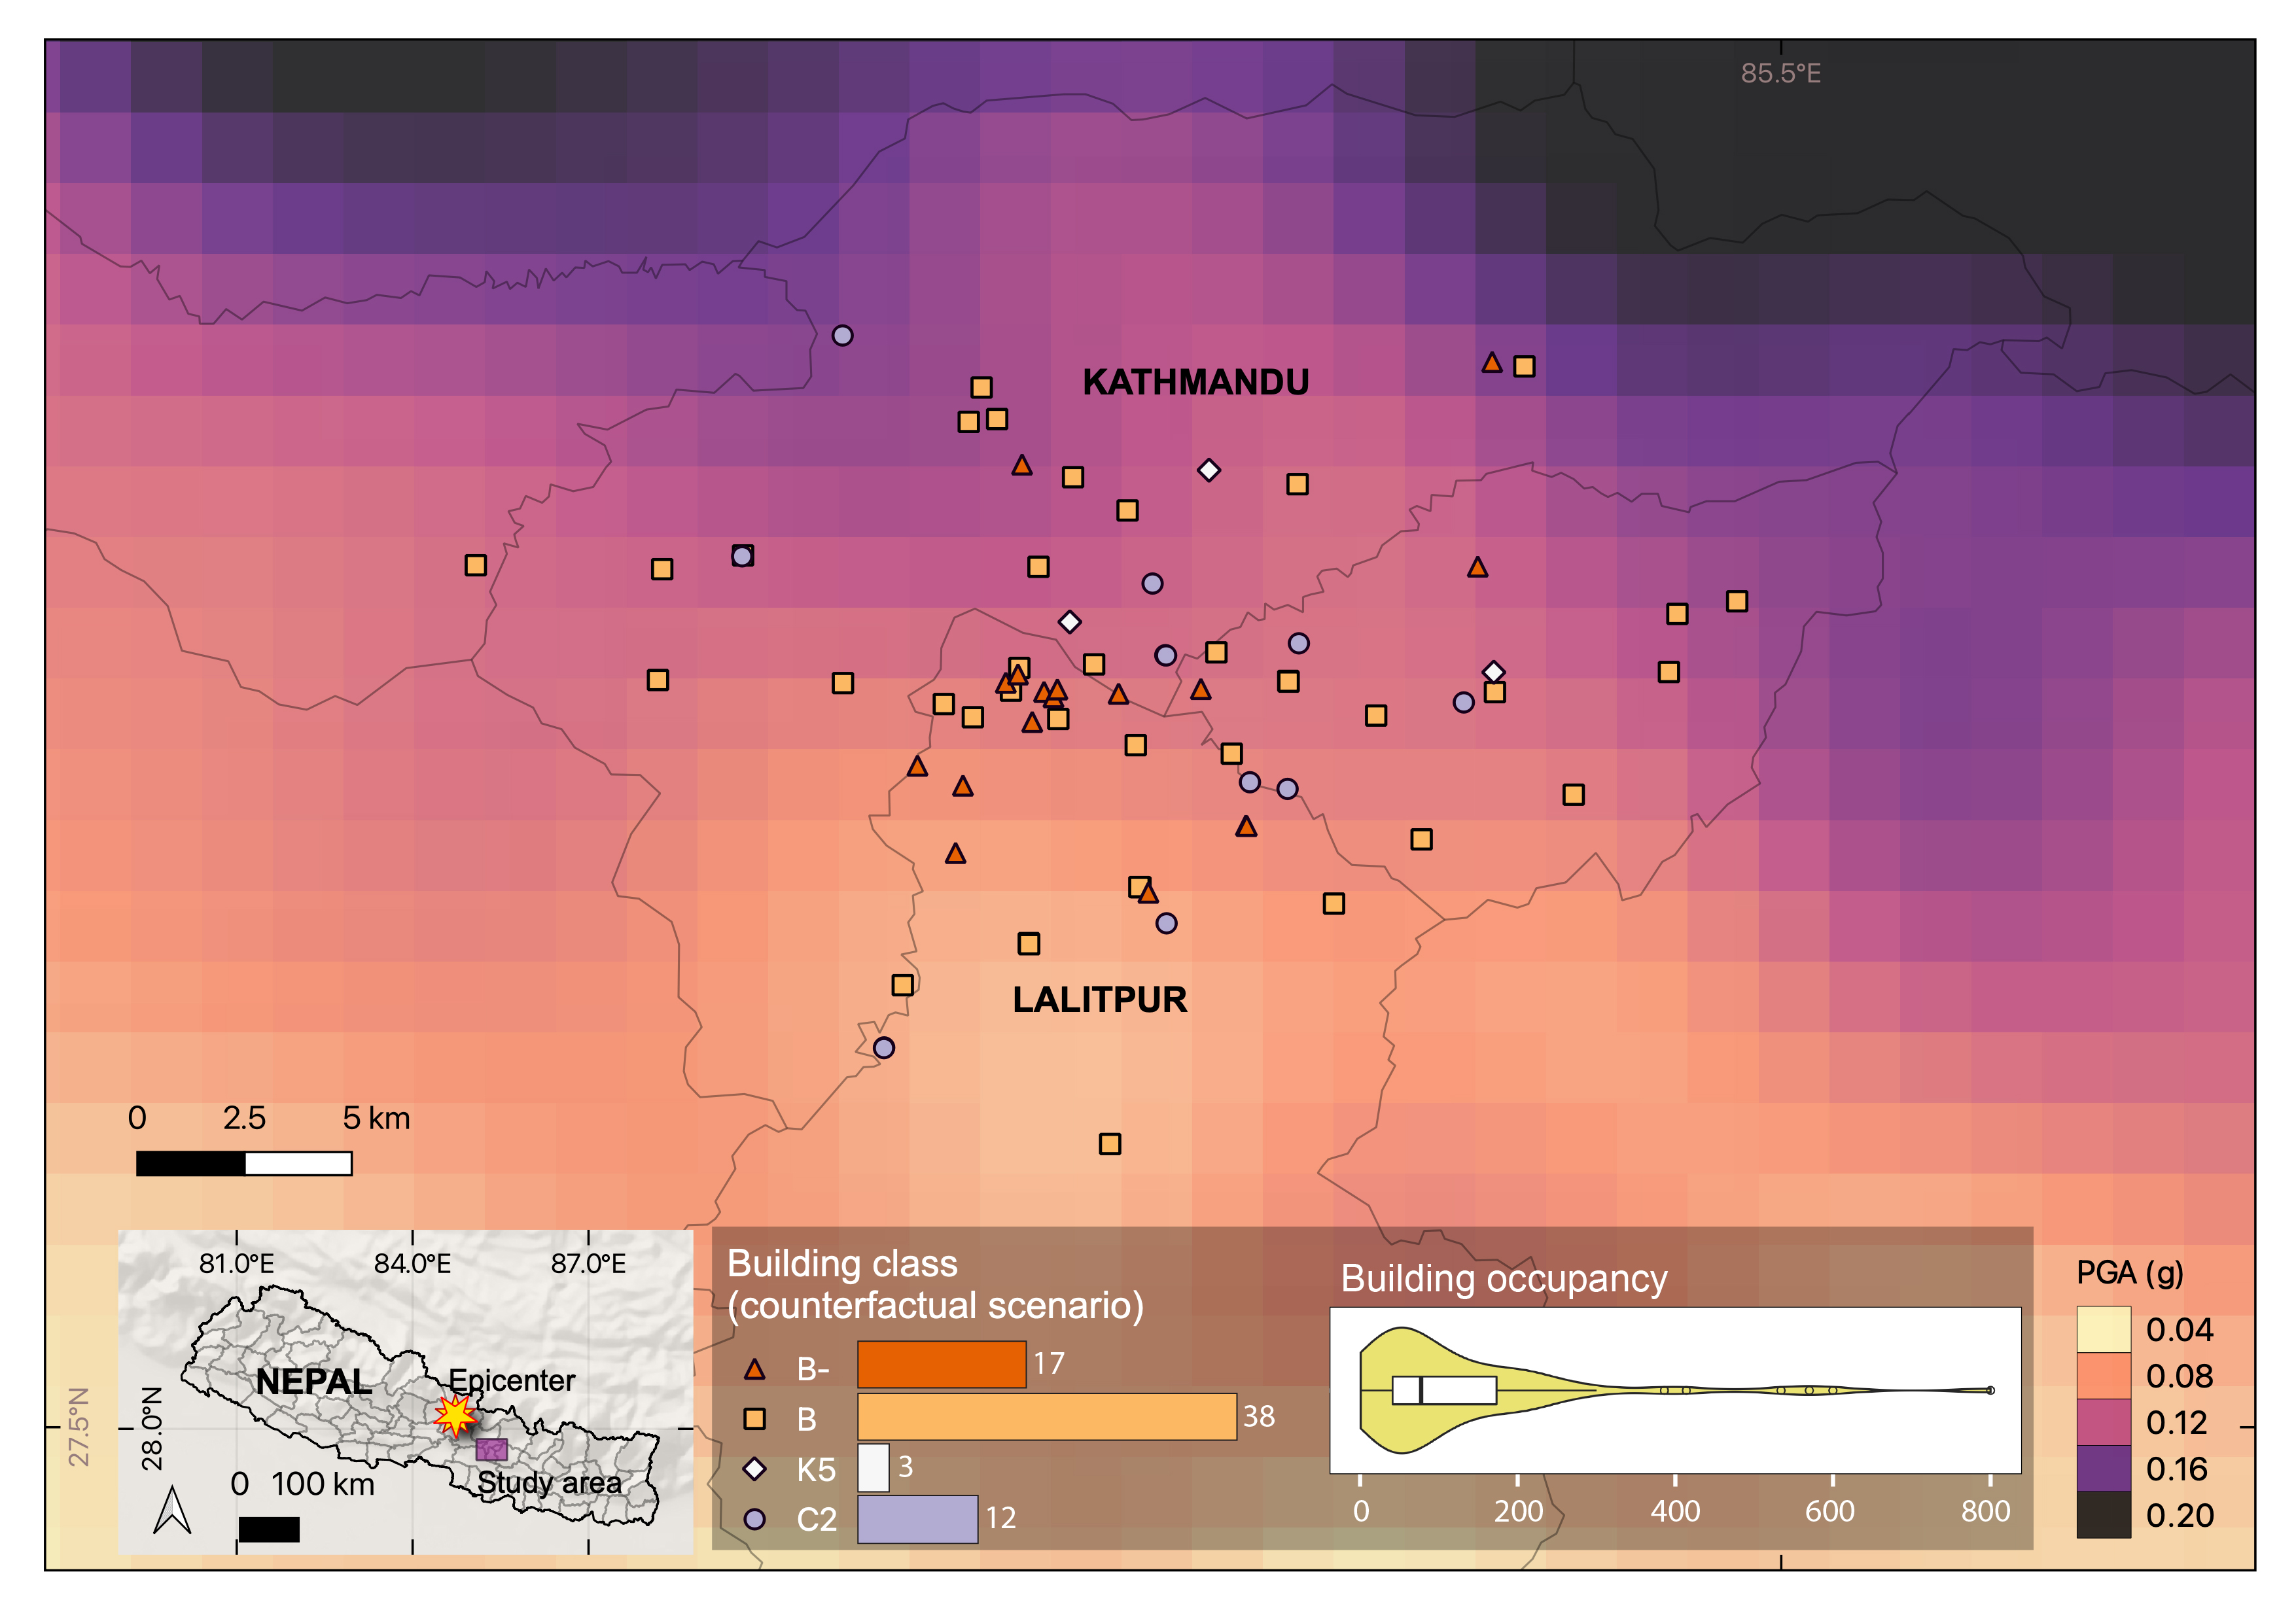
\includegraphics[width=\linewidth]{Figures/data-case1.jpg}
	\caption{Datasets used for the case study in Section \ref{section-case1} to estimate the lives saved by the retrofitting of 70 schools amidst the 2015 Gorkha earthquake. For the realised scenario, all the 70 retrofitted school buildings shown on the map are assigned as building class C3. For the counterfactual scenario, all buildings were assumed to be non-retrofitted and assigned to building classes shown in the bar graph at the bottom. The buildings’ daytime occupants range from 1 to 800 with distribution as a violin plot at the bottom. The basemap shows the peak ground acceleration (in g-units) adopted from \cite{chen20192015}.}
	\label{fig:datacase1}
\end{center}
\end{figure}

\begin{figure}[h!]
\begin{center}
     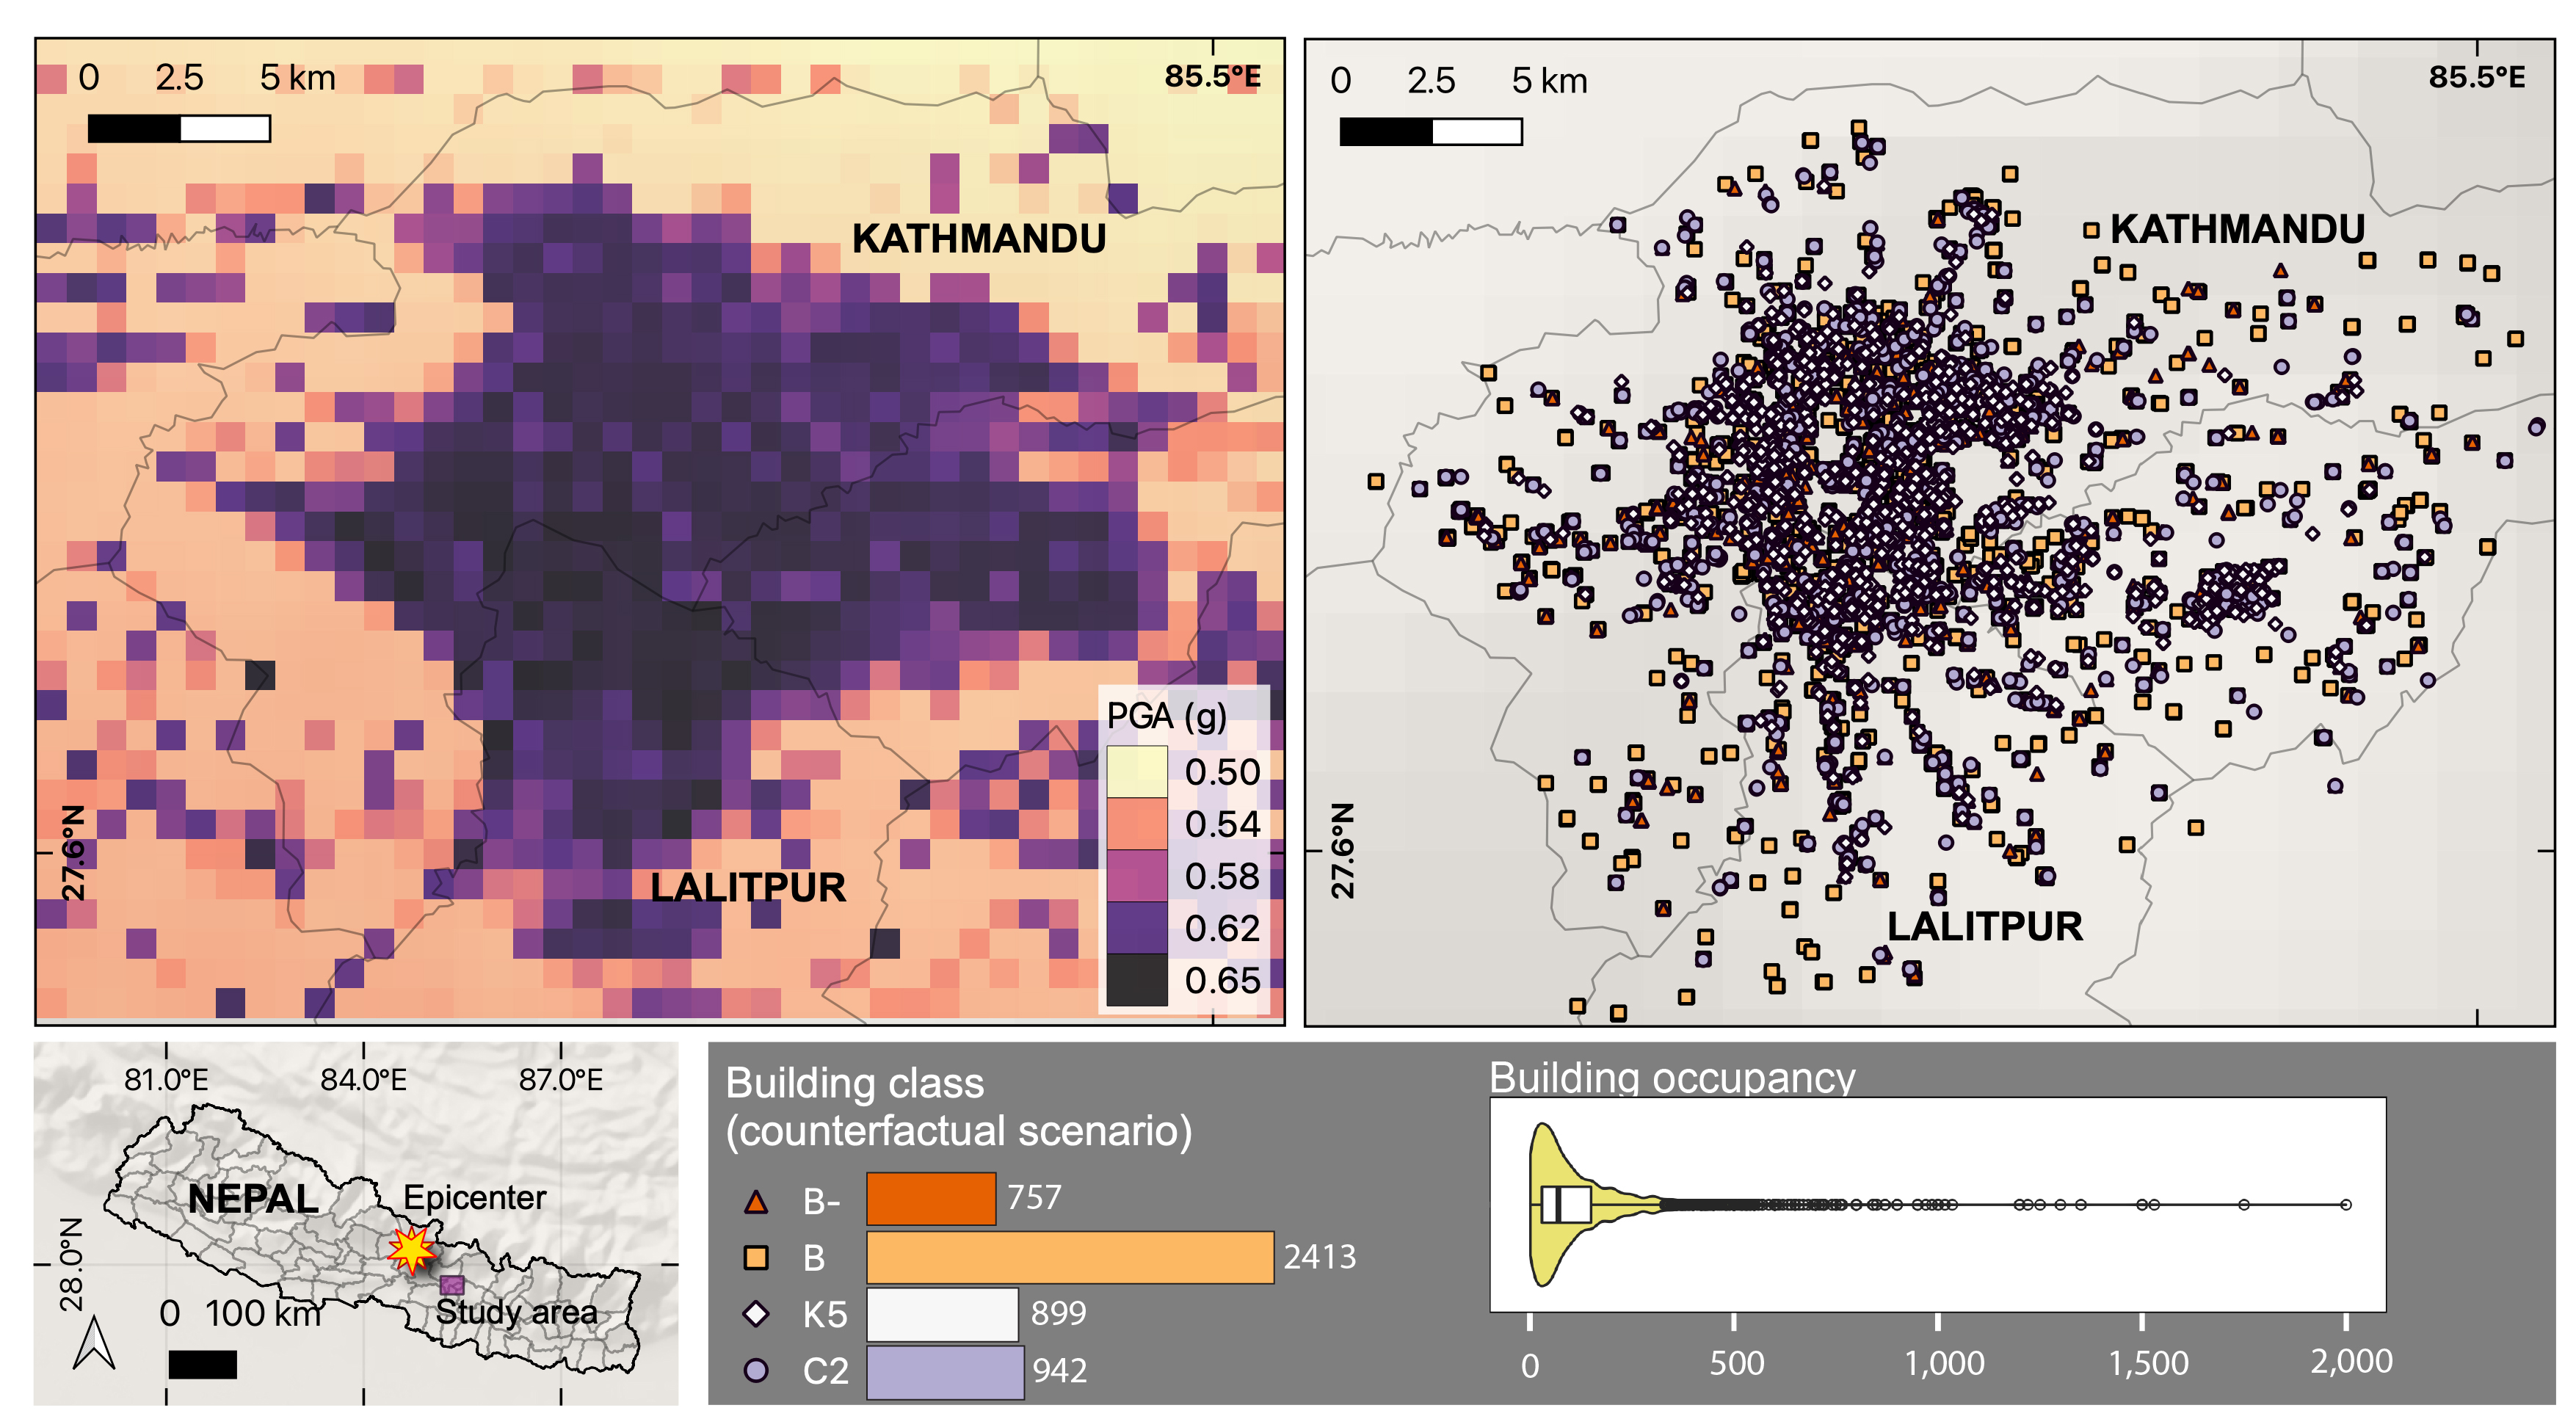
\includegraphics[width=\linewidth]{Figures/data-case2.jpg}
		\caption{Datasets used for the case study in Section \ref{section-case2} to forecast the lives saved by the retrofitting of the 5,011 school buildings in the event of a 10\% in 50 years shaking. Shown in the top left is a map of PGA in g-units generated by \cite{stevens2018probabilistic} for 10\% exceedance in 50 year shaking. The location of the 5,011 retrofitted school buildings are shown in the top right. For the realised scenario, all buildings were retrofitted and categorized as building class C3. For the counterfactual scenario, all buildings were assumed to be non-retrofitted and assigned to building classes shown in the bar graph at the bottom. The buildings’ daytime occupants range from 1 to 2000 with distribution as a violin plot at the bottom.}
	\label{fig:datacase2}
\end{center}
\end{figure}
    
\begin{figure}[h!]
\begin{center}
    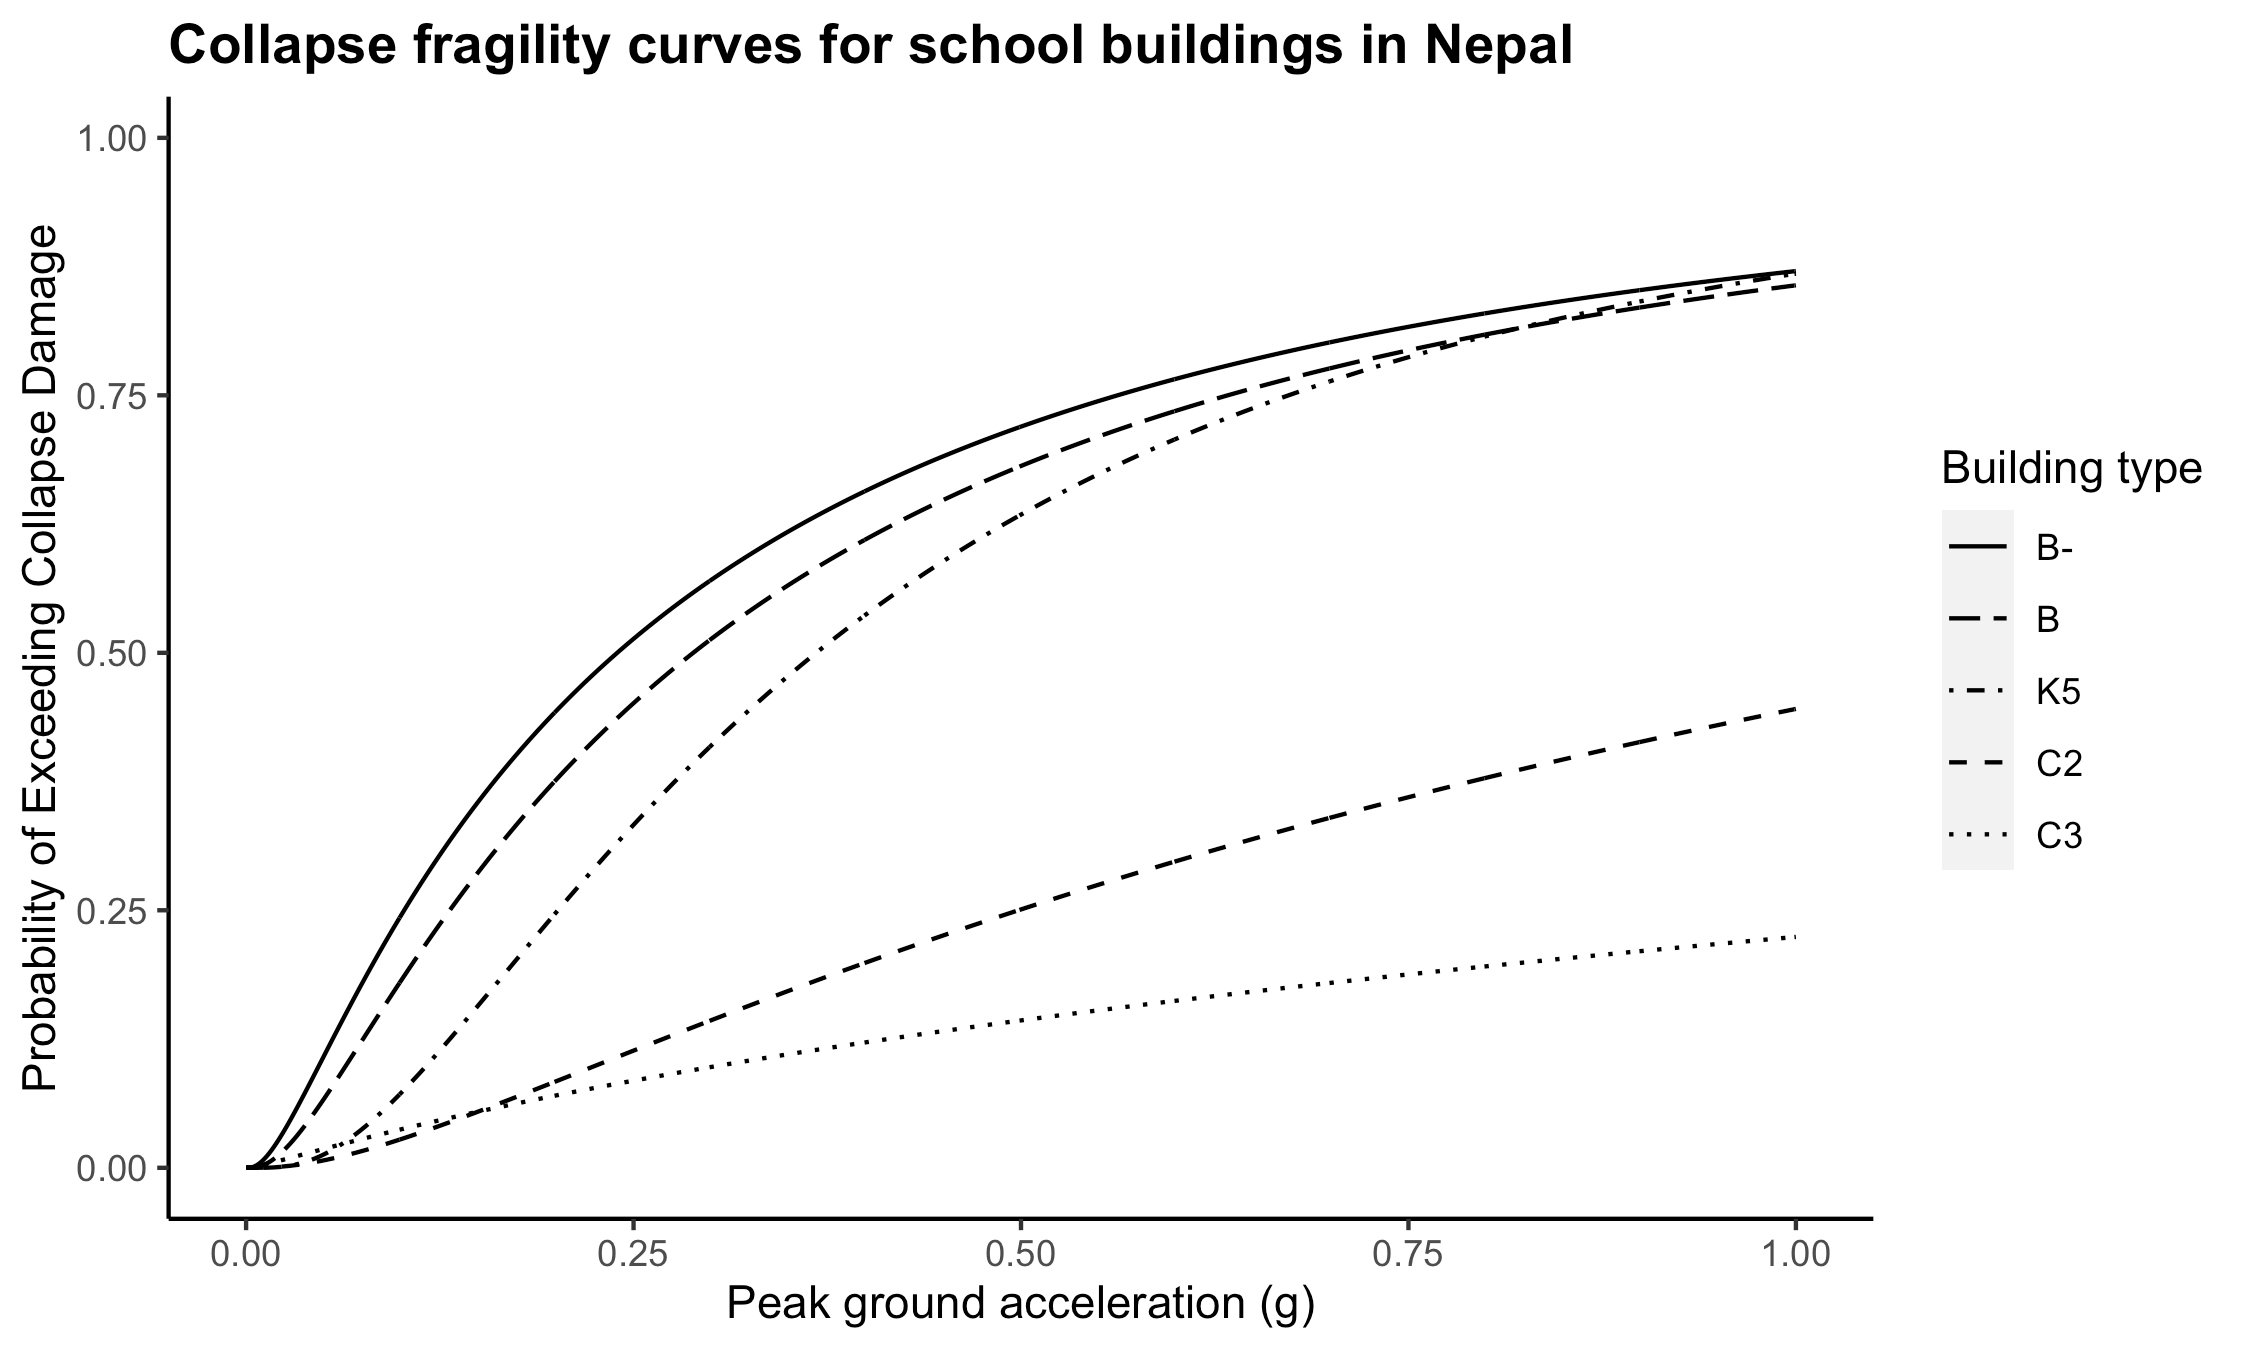
\includegraphics[width=\linewidth]{Figures/data-fragility.jpg}
    \caption{Collapse fragility curves for the building classes in the full building portfolio adopted from \citep{jica2002study}. Non-retrofitted building classes include B-, B, K5, and C2, while the retrofitted buildings are assigned as type C3. Refer to Table \ref{tab:frag_params} for complete descriptions of building classes.}
    \label{fig:frag_curves}
\end{center}
\end{figure}

\begin{figure}[h!] 
\begin{center} 
    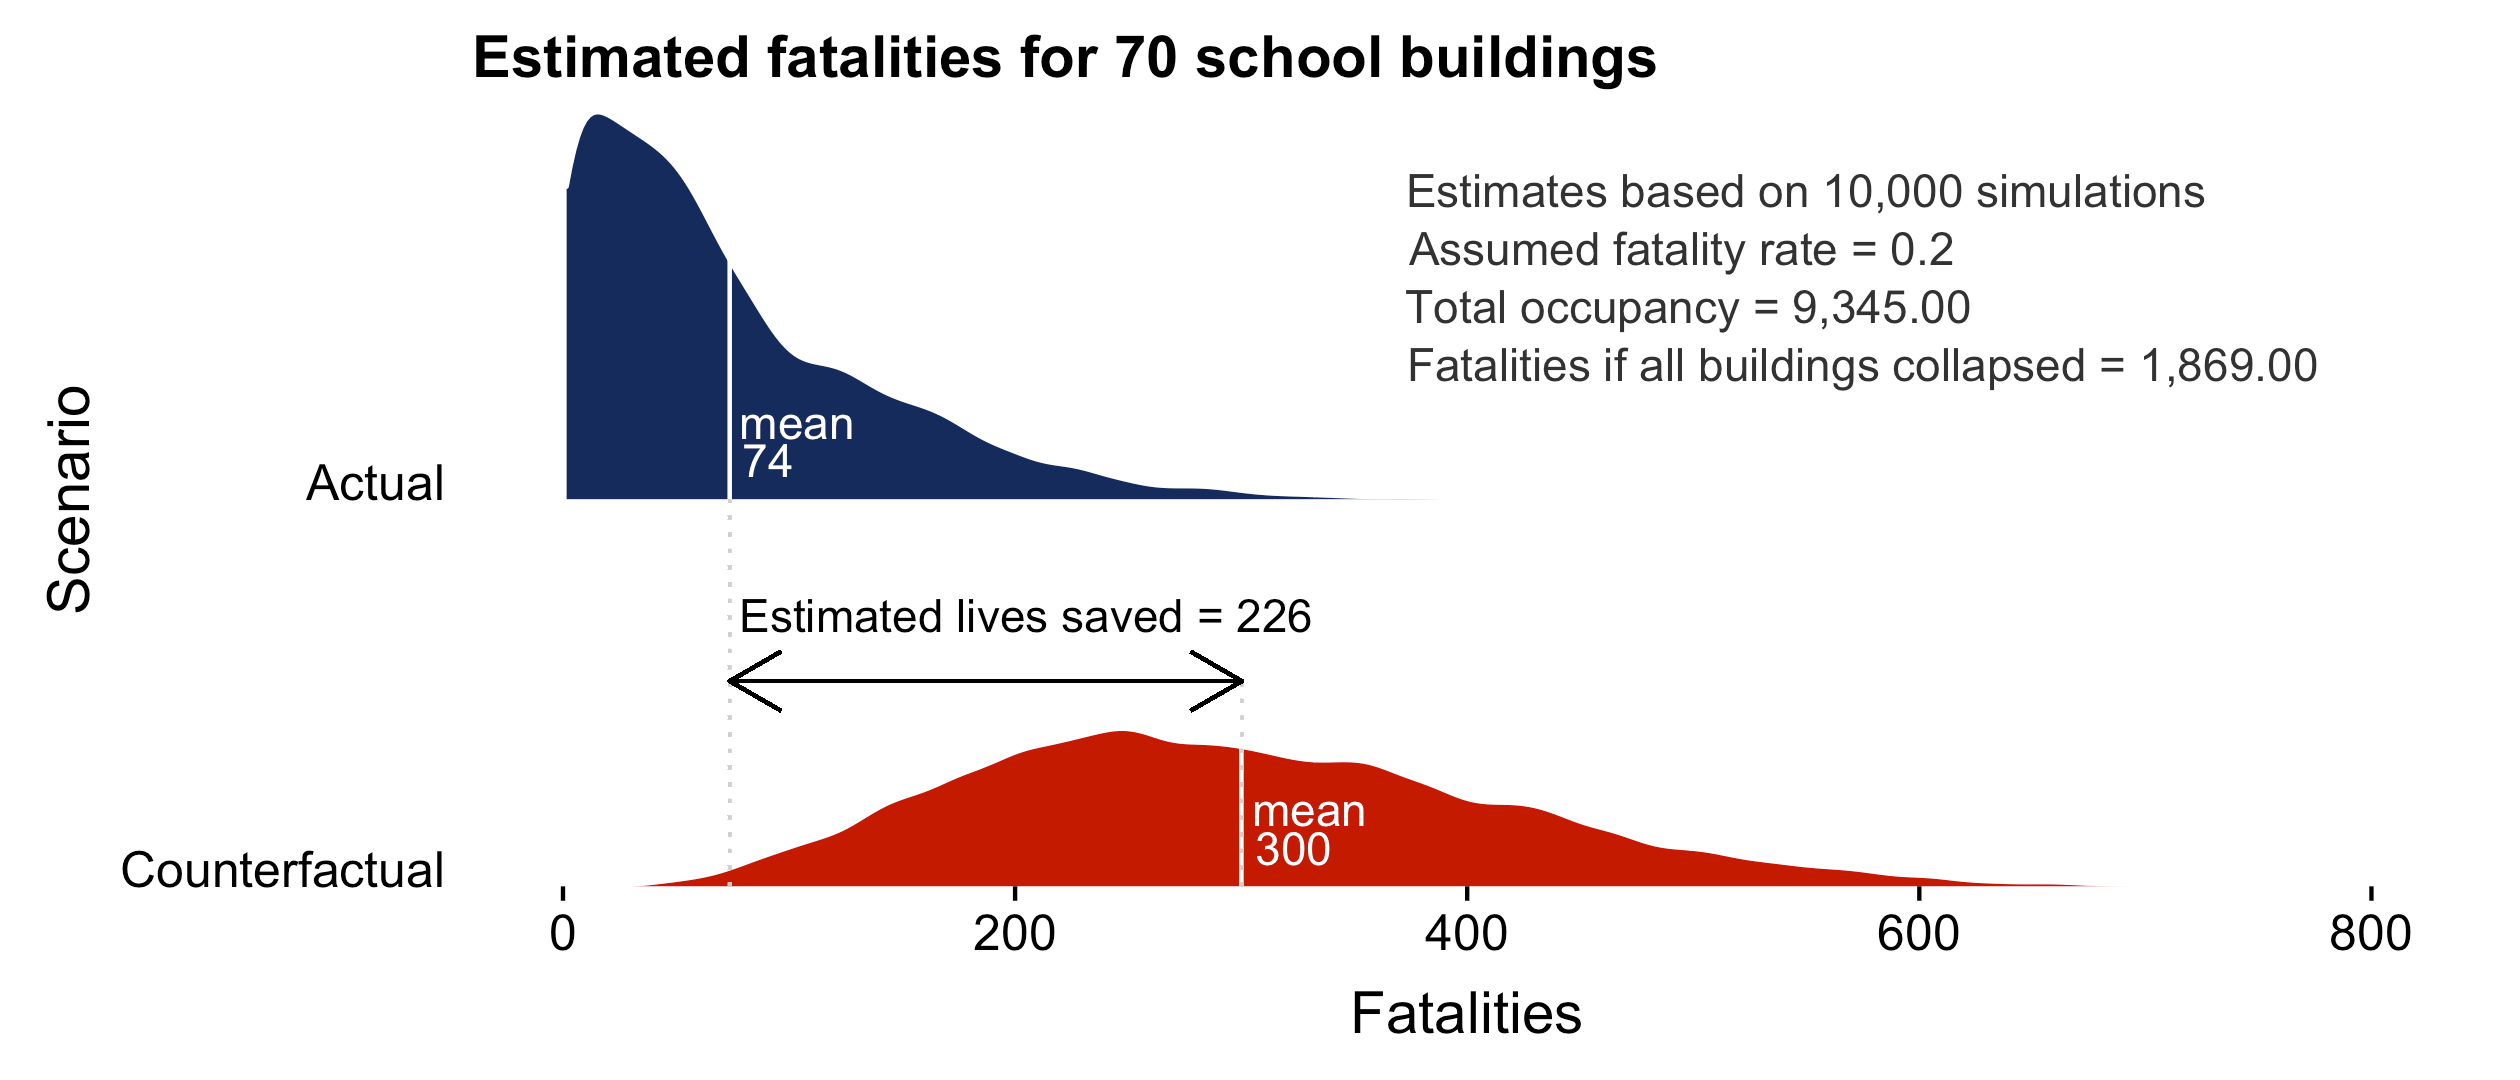
\includegraphics[width=\linewidth]{Figures/results-case1.jpg}
	\caption{Distribution of estimated fatalities from the 2015 $M_{w}$ 7.8 Gorkha earthquake based on earthquake intensity values from \cite{chen20192015}. Two scenarios are shown: the actual scenario where all 70 school buildings were retrofitted prior to the 2015 Gorkha earthquake, and a counterfactual scenario where the schools were not retrofitted.  The difference between the means of the actual and counterfactual scenario represent the estimated lives saved by the retrofit program. In reality, none of the 70 school buildings collapsed after the Gorkha earthquake. Our probabilistic analysis show an estimated 226 lives saved by the schools retrofit program during the Gorkha earthquake.}
\label{fig:results_case1}
\end{center}
\end{figure}

\begin{figure}[h!]
\begin{center} 
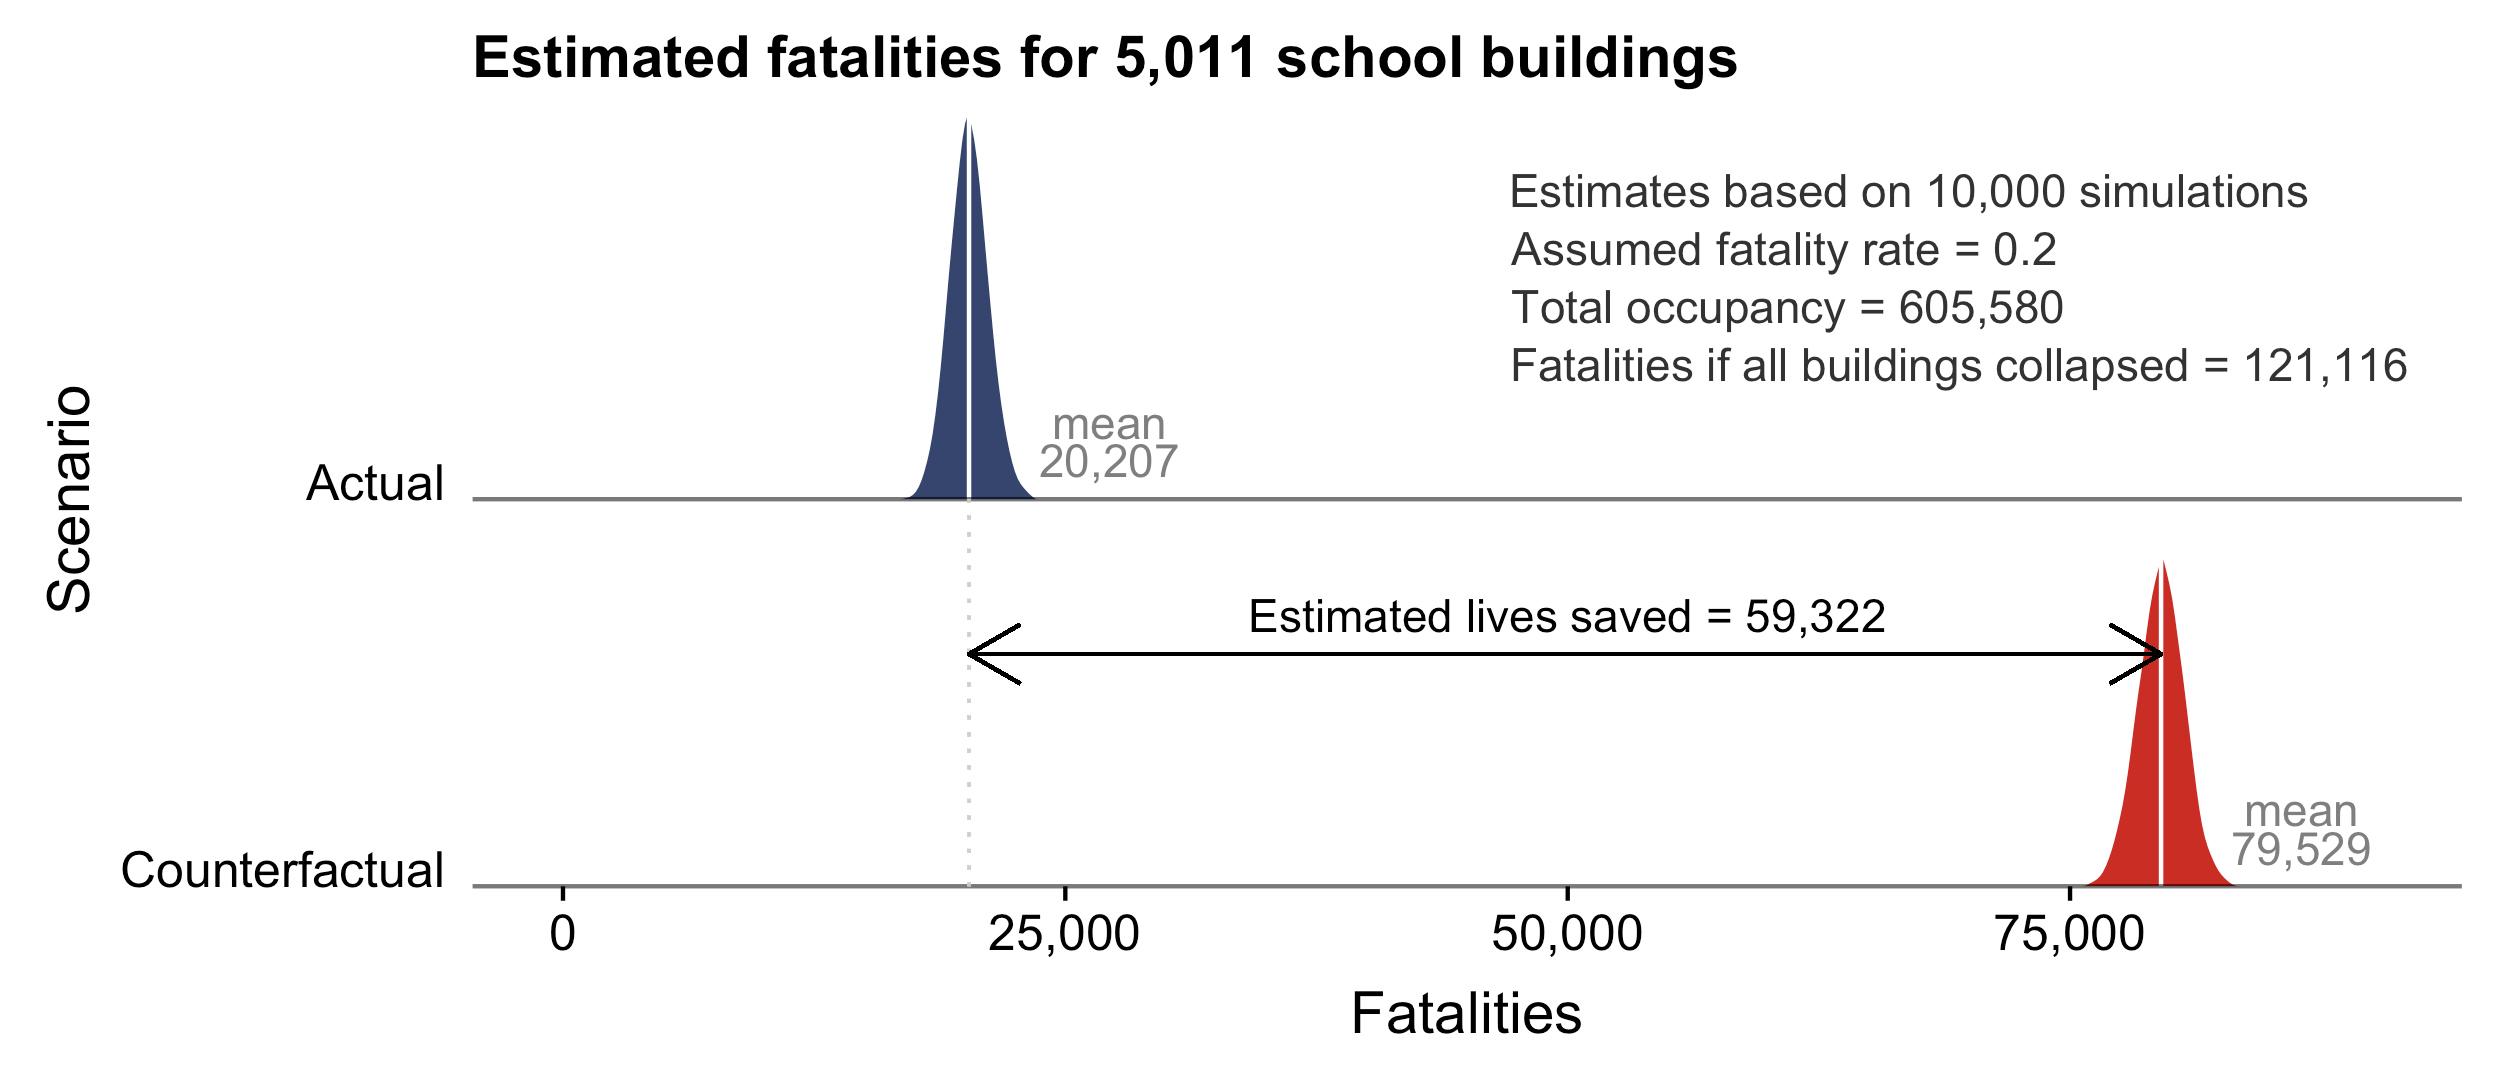
\includegraphics[width=\linewidth]{Figures/results-case2.jpg}
	\caption{Distributions of estimated fatalities based on PGA values for 10\% probability of exceedance in 50 years from \cite{stevens2018probabilistic}. In the actual scenario, all 5,011 school buildings (See Figure \ref{fig:datacase2}) were completely retrofitted. For the counterfactual scenario, all school buildings were not retrofitted (i.e. the intervention doesn't exist). Our probabilistic analysis show that retrofitting all 5,011 school buildings will likely save 59,322 lives in the event of a 10\% in 50 years shaking.}
\label{fig:results_case2}
\end{center}
\end{figure}

%%%TABLE
% Please add the following required packages for this table:
% \usepackage{multirow, graphicx}
\begin{table}[]
\caption{Building classes for schools in Nepal and associated fragility curve parameters. (Data source: \citep{opendri_2012, jica2002study}}
\label{tab:frag_params}
\resizebox{\textwidth}{!}{%
\begin{tabular}{|c|l|c|c|c|}
\hline
    \multirow{2}{*}{\begin{tabular}[c]{@{}c@{}}Building \\ type\end{tabular}} &
    \multicolumn{1}{c|}{\multirow{2}{*}{Description}} &
    \multirow{2}{*}{\begin{tabular}[c]{@{}c@{}}Structural state \\ of building\end{tabular}} &
    \multicolumn{2}{c|}{\begin{tabular}[c]{@{}c@{}}Fragility curve \\ parameters\end{tabular}} \\ \cline{4-5} 
        & \multicolumn{1}{c|}{}   &   & $\alpha$  & $\beta$  \\ \hline
    \rule{0pt}{3ex}%  EXTRA vertical height  
            
    B- &
    \begin{tabular}[c]{@{}l@{}}B-type rural buildings with traditional materials\\ and height up to three storeys, or with cement mortar\\ in brick masonry and height up to five storeys.\end{tabular} &
        Un-retrofitted &
        1.129 &
        0.790 \\ \hline
    \rule{0pt}{3ex}%  EXTRA vertical height  
            
            
    B &
    \begin{tabular}[c]{@{}l@{}}Buildings with mud mortar, ordinary brick,\\ large blocks, natural dressed stone with height\\ up to 1 storey, or with cement mortar in brick masonry\\ and height up to 3 storeys.\end{tabular} &
        Un-retrofitted &
        1.066 &
        0.858 \\ \hline
    \rule{0pt}{3ex}%  EXTRA vertical height    
            
    K5 & Mason-designed 5 storey RC buildings & Un-retrofitted & 1.118  & 1.246 \\ \hline
    \rule{0pt}{3ex}%  EXTRA vertical height  

    C2 &
    \begin{tabular}[c]{@{}l@{}}Reinforced buildings (RC) designed for normal load only, or\\ mason designed 3 storey RC buildings.\end{tabular} &
        Un-retrofitted &
        -0.137 &
        0.772 \\ \hline
    \rule{0pt}{3ex}%  EXTRA vertical height  
            
    C3 & Specially designed RC buildings      & Retrofitted    & -0.758 & 0.445 \\ \hline

\end{tabular}%
}
\end{table}            


%%% Please be aware that for original research articles we only permit a combined number of 15 figures and tables, one figure with multiple subfigures will count as only one figure.
%%% Use this if adding the figures directly in the mansucript, if so, please remember to also upload the files when submitting your article
%%% There is no need for adding the file termination, as long as you indicate where the file is saved. In the examples below the files (logo1.eps and logos.eps) are in the Frontiers LaTeX folder
%%% If using *.tif files convert them to .jpg or .png
%%%  NB logo1.eps is required in the path in order to correctly compile front page header %%%
%%% If you are submitting a figure with subfigures please combine these into one image file with part labels integrated.
%%% If you don't add the figures in the LaTeX files, please upload them when submitting the article.
%%% Frontiers will add the figures at the end of the provisional pdf automatically
%%% The use of LaTeX coding to draw Diagrams/Figures/Structures should be avoided. They should be external callouts including graphics.

%%%% SAMPLE CAPTION
% \begin{figure}[h!]
% \begin{center}
% \includegraphics[width=10cm]{logo1}% This is a *.eps file
% \end{center}
% \caption{ Enter the caption for your figure here.  Repeat as  necessary for each of your figures}\label{fig:1}
% \end{figure}

%%%% SAMPLE CAPTION - WITH SUBFIGURES
% \begin{figure}[h!]
% \begin{center}
% \includegraphics[width=15cm]{logos}
% \end{center}
% \caption{This is a figure with sub figures, \textbf{(A)} is one logo, \textbf{(B)} is a different logo.}\label{fig:2}
% \end{figure}



%%%%%%%%%%%%%%%%%%%%%%%%%%%%
\end{document}
%%%%%%%%%%%%%%%%%%%%%%%%%%%%%%%%%%%%%%%%%%%%%%%%%%%%%%%%


%%%%%%%%%%%%%%%%%%%%%%%%%%%%%%%%%%%%%%%%%%%%%%%%%%%%%%%%
%%% TEMPLATE GUIDELINE
%%%%%%%%%%%%%%%%%%%%%%%%%%%%%%%%%%%%%%%%%%%%%%%%%%%%%%%%

% \section{Introduction}
% For Original Research Articles \citep{conference}, Clinical Trial Articles \citep{article}, and Technology Reports \citep{patent}, the introduction should be succinct, with no subheadings \citep{book}. For Case Reports the Introduction should include symptoms at presentation \citep{chapter}, physical exams and lab results \citep{dataset}.

% \section{Article types}
% For requirements for a specific article type please refer to the Article Types on any Frontiers journal page. Please also refer to  \href{http://home.frontiersin.org/about/author-guidelines#Sections}{Author Guidelines} for further information on how to organize your manuscript in the required sections or their equivalents for your field
% For Original Research articles, please note that the Material and Methods section can be placed in any of the following ways: before Results, before Discussion or after Discussion.

% \section{Manuscript Formatting}
% \subsection{Heading Levels}
% %There are 5 heading levels
%     \subsection{Level 2}
%     \subsubsection{Level 3}
%     \paragraph{Level 4}
%     \subparagraph{Level 5}
    
% \subsection{Equations}
% Equations should be inserted in editable format from the equation editor.
%     \begin{equation}
%     \sum x+ y =Z\label{eq:01}
%     \end{equation}

% \subsection{Figures}
% Frontiers requires figures to be submitted individually, in the same order as they are referred to in the manuscript. Figures will then be automatically embedded at the bottom of the submitted manuscript. Kindly ensure that each table and figure is mentioned in the text and in numerical order. Figures must be of sufficient resolution for publication \href{http://home.frontiersin.org/about/author-guidelines#ResolutionRequirements}{see here for examples and minimum requirements}. Figures which are not according to the guidelines will cause substantial delay during the production process. Please see \href{http://home.frontiersin.org/about/author-guidelines#GeneralStyleGuidelinesforFigures}{here} for full figure guidelines. Cite figures with subfigures as figure \ref{fig:2}B.